\section{Implementation}												
\label{sec:Implementation}

\paragraph{}For the Android application, Android and Java were chosen as the primary programming languages due to the developer's familiarity with them. For the web interface, JSP was chosen as the background language. JavaScript and HTML were chosen to take care of the front-end and user interface. Ajax is also used to talk to the database. 

\subsection{Bmob Usage}
\label{subsec:DatabaseOperations}
\paragraph{}As we mentioned in the design section, the Bmob online database was chosen for the database management system (DBMS) for both the Android application and the web interface. To use this database, we need an entity class to match each table. The entity class must extend {\ttfamily BmobObject} and the class name must be the same as the table name. For example, the friend class is shown below:

\begin{center}
\begin{lstlisting}[caption={Friend Class},language={java},
        numbers=left,basicstyle=\footnotesize\ttfamily,xleftmargin=.2\textwidth, xrightmargin=.2\textwidth]
public class Friend extends BmobObject {
    private String user;
    private String friend;
    public String getUser() {
        return user;
    }
    public void setUser(String user) {
        this.user = user;
    }
    public String getFriend() {
        return friend;
    }
    public void setFriend(String friend) {
        this.friend = friend;
    }
}
\end{lstlisting} 
\end{center}


\begin{figure}[htb]
\centering
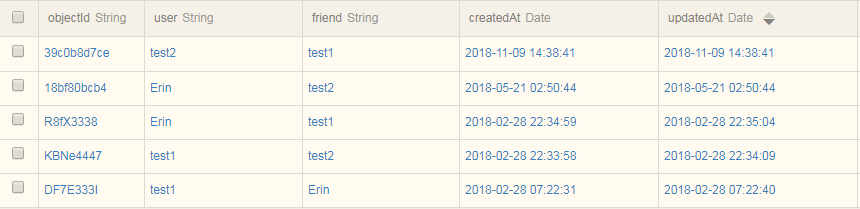
\includegraphics[width=1\textwidth]{section04/assets/databaseOverview.png}
\caption[Table Friend]{\label{DatabseOverview}Table \bsq{Friend}}
\end{figure}
\par Figure \ref{DatabseOverview} is the corresponding table in the database. The \bsq{\ttfamily objectId},\bsq{\ttfamily createdAt} and \bsq{\ttfamily updatedAt} columns are generated by Bmob automatically. 
\par After we wrote the entity classes, we then needed to use them in the application. Three steps are needed for usage: 
\begin{enumerate}
\item[1)]Import SDK into your app level build.gradle file like this:
\begin{lstlisting}[caption={Import Bmob},language={java},
        basicstyle=\footnotesize\ttfamily,xleftmargin=.1\textwidth, xrightmargin=.2\textwidth]
implementation 'cn.bmob.android:bmob-sdk:3.6.3'
\end{lstlisting} 
\item[2)] Configure the {\ttfamily AndroidManifest.xml} file. This file is used to declare an application component and declare the permissions that the application needs. We will include this in later subsection \ref{subsubsec:GetSystemPermissions} Get System Permissions.
\item[3)] Initialize the BmobSDK. The BmobSDK uses APIKeys to ensure that a REST API call is valid.  The initialization processes links the APIKey to all REST API calls made by the SDK. 

\end{enumerate}
\par After initialization is finished. We can get access to the database like this:
\begin{lstlisting}[caption={Bmob Query Example},            language={java}, numbers=left, basicstyle=\footnotesize\ttfamily,breaklines=true,xleftmargin=.15\textwidth, xrightmargin=.2\textwidth]
BmobQuery<User> query = new BmobQuery<>();
query.addWhereEqualTo("username", username);
query.findObjects(new FindListener<User>() {
    @Override
    public void done(List<User> users, BmobException e) {
        if(e == null){
            saveProfile(users.get(0),newPassword);
        }else{
            Log.i("bmob","failed:"+e.getMessage()+","+
            e.getErrorCode());
        }
    }
});
\end{lstlisting} 
\par All the data operations have a template which makes it easier to perform database operations. An inner class will be needed for each database operation. The above code shows how to retrieve data from Bmob and is a pattern used throughout the application. Line 2 adds a constraint for the query which is the value of \bsq{\ttfamily username} column equals the String username. The \bsq{\ttfamily users} in Line 5 will save the result if the query succeeded. If the error message, {\ttfamily e}, is null, then it means the query succeeded. 

\subsection{Image Processing Algorithms with OpenCv}
\paragraph{}This project addresses two central problems about image processing: transforming the gift image to fit in user selected regions and finding the correct region when users receive the gift. We use OpenCv to help finish these functions. OpenCV is a cross-platform library which we can use to develop real-time computer vision applications. It mainly focuses on image processing, video capture and analysis including features like face detection and object detection. For this project we mainly use the \bsq{\ttfamily Features2D} class to transform the gift image and find keypoints and matches. Then use \bsq{\ttfamily Homography} to identify a target region in a real-time image. 

\subsubsection{Sending a Gift}
\paragraph{} To send a gift, the user captures an image with their smart phone.  When the image is captured, the GPS coordinates are also recorded for later use.  The user must then identify what region of the captured image they would like for the gift to appear.  The user selects the region by dragging four corners of a quadrilateral that form the boundaries of the gift image to be projected onto and overlayed on top of the captured image.
\par After the user selects a region and a gift image, the gift needs to fit the shape of the region and we made a perspective transformation on the selected gift and then apply this transformation to the user selected region. 
\begin{figure}[htb]
\centering
\begin{minipage}[H]{0.3\textwidth}

\includegraphics[width=.95\textwidth]{section04/assets/OriginalGift.png}
\subcaption{\label{OriginalGift}}
\end{minipage}%
\begin{minipage}[H]{0.3\textwidth}
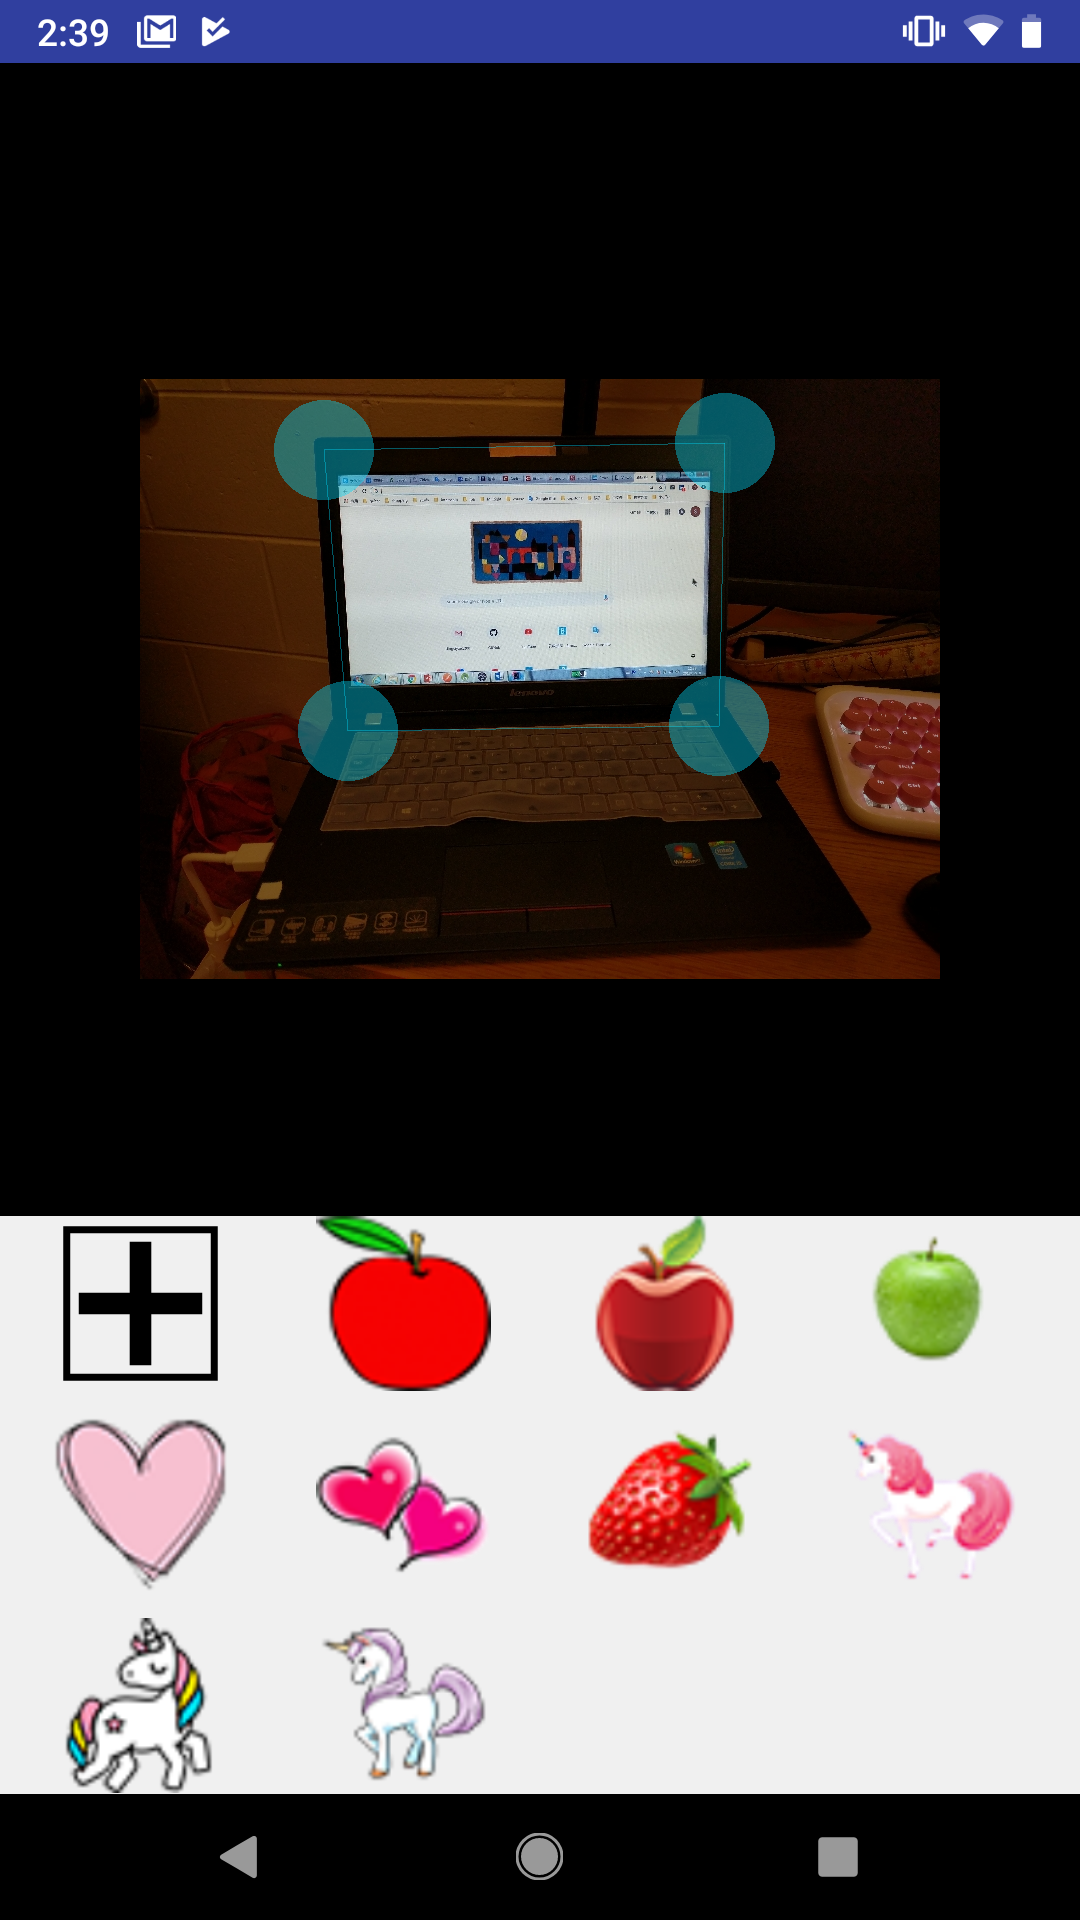
\includegraphics[width=.95\textwidth]{section04/assets/GiftThransformExample.png}
\subcaption{\label{GiftThransformExample}}
\end{minipage}%
\begin{minipage}[H]{0.3\textwidth}
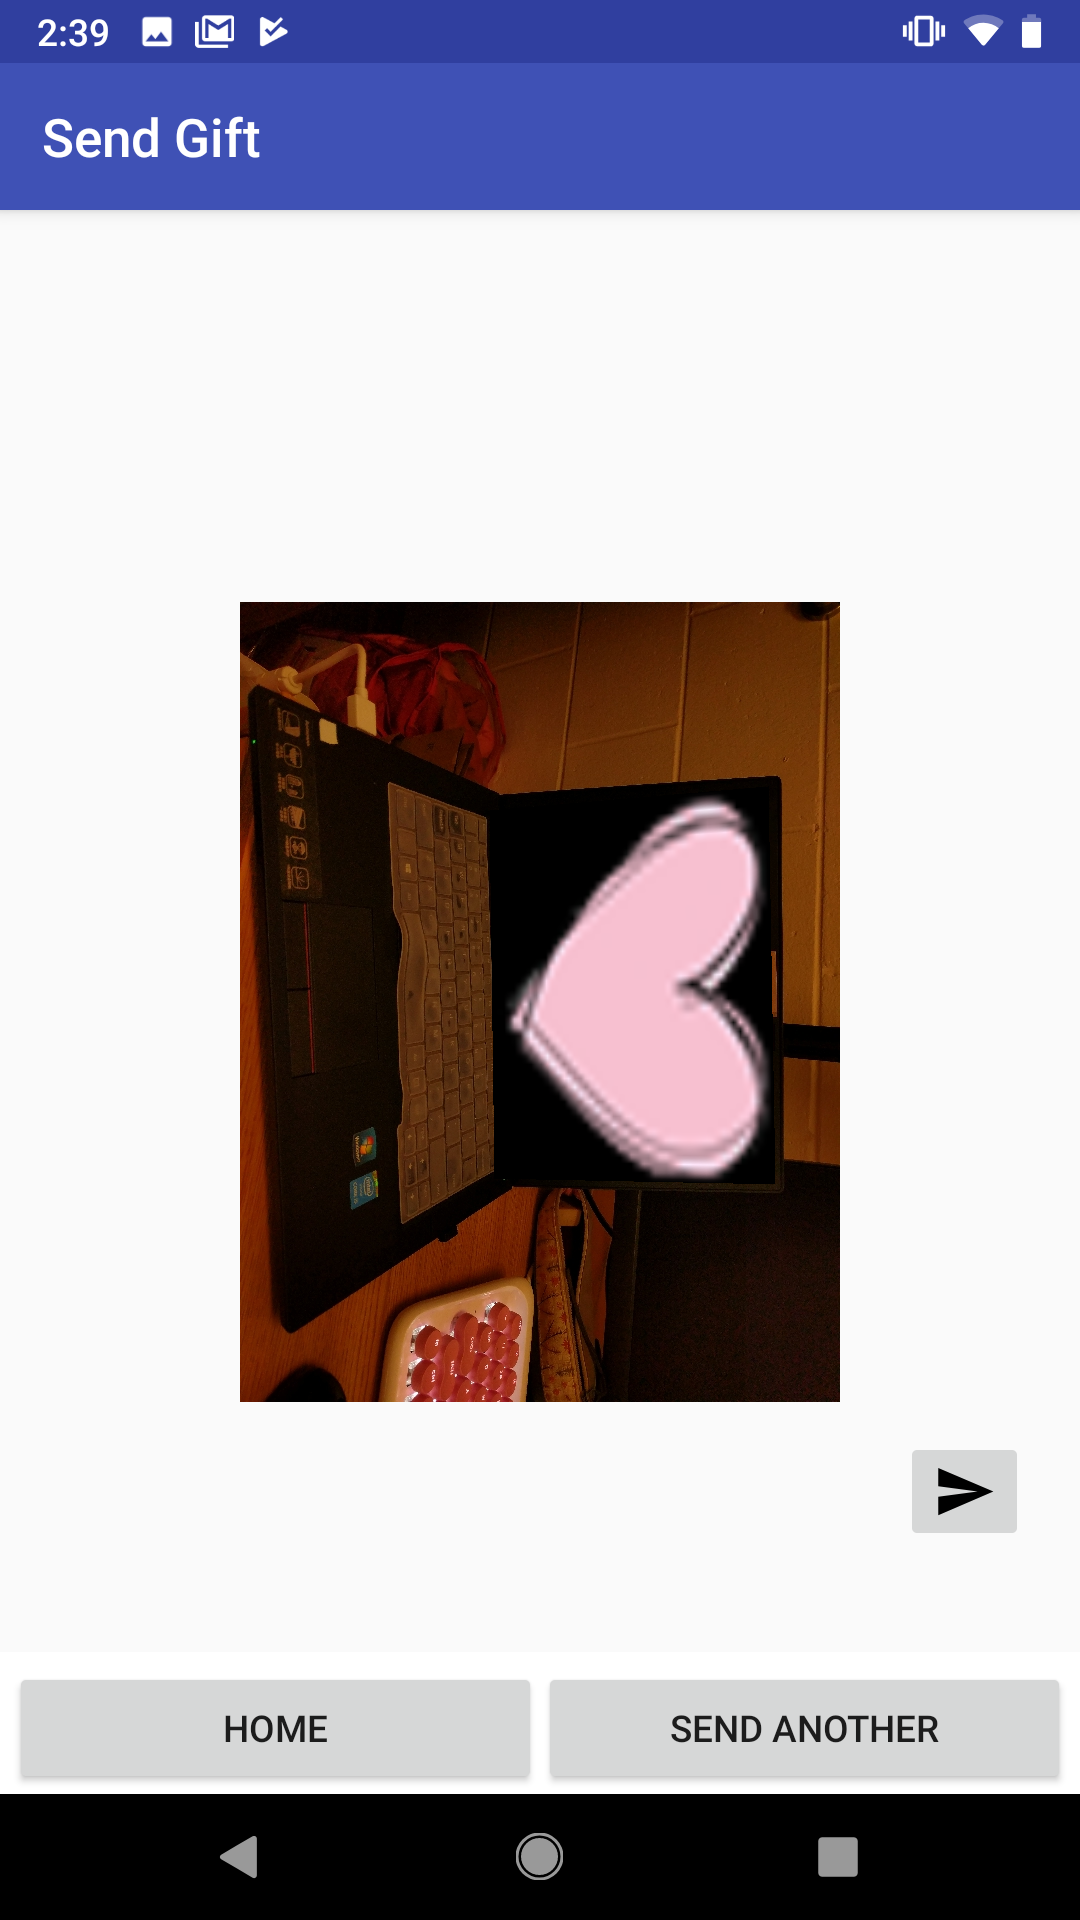
\includegraphics[width=.95\textwidth]{section04/assets/AttachedGift.png}
\subcaption{\label{AttachedGift}}
\end{minipage}%
\caption[Gift Transformation Example]{\label{GiftTransformationExample}Gift Transformation Example}
\end{figure}
\par The process is shown in Figure \ref{GiftTransformationExample}. As we can see, Figure \ref{OriginalGift} shows the gift which will be attached to the user selected region. Figure \ref{GiftThransformExample} shows the user selected region on the captured image. This region must be a four sided shape and the application will correct it automatically if the user drags corners such that the corners must be rearranged. After we selected a region and gift image, the gift will be mapped to the user-selected region and will be overlayed on top of the region as shown in Figure \ref{GiftTransformationExample}.
\par The following code shows how we do the perspective transformation. For perspective transformation, we use a 3x3 transformation matrix. To find this transformation matrix, we need four points on the gift image which will be the four corners of the gift image and corresponding points on the background image. The corresponding points will be the four corners of the user selected region.  Among these four points, three of them should not be collinear. Then transformation matrix can be found by the function getPerspectiveTransform at Line 15. Then use the warpPerspective function at Line 16  to apply transformation with this 3x3 transformation matrix. The code below is the method used to apply transformation, drawable is the gift image, region is the background image, points contains the four corners user selected.

\begin{lstlisting}[caption={Gift Transform},language={java},
        numbers=left,basicstyle=\footnotesize\ttfamily,breaklines=true,xleftmargin=.1\textwidth, xrightmargin=.1\textwidth]
Mat getThansform(Mat drawable, Mat region, int[] points) {
    Mat drawableCorner = 
        new Mat(4, 1, CvType.CV_32FC2);
    Mat drawableTransformCorner = 
        new Mat(4, 1, CvType.CV_32FC2);

    drawableCorner
        .put(0, 0, new double[]{0.0, 0.0});
    drawableCorner
        .put(1, 0, new double[]{drawable.cols(), 0.0});
    drawableCorner
        .put(2, 0, new double[]{ 
            drawable.cols(), drawable.rows()
        });
    drawableCorner
        .put(3, 0, new double[]{
            0.0, drawable.rows()
        });
    
    for(int i=0; i<4; i++){
        drawableTransformCorner.put(i, 0, new double[]{points[i*2], points[i*2+1]});
    }

    Mat perspectiveTransform = Imgproc.getPerspectiveTransform(drawableCorner, drawableTransformCorner);
    Imgproc.warpPerspective(drawable,region,perspectiveTransform, region.size(), Imgproc.INTER_LINEAR,
    Core.BORDER_TRANSPARENT, new Scalar(0, 0, 0, 0));

    return region;
}
\end{lstlisting} 
\subsubsection{Finding a Gift}
\paragraph{}
When a user receives a gift, they must go to the GPS coordinates attached to the gift.  Once in the approximate vicinity, they must scan the area with their smart phone in order to find the image that the sender captured along with the sender-selected region. Once the region is recognized, the gift image will appear to the recipient. This image recognition process is computationally challenging.

\par Image recognition is accomplished in OpenCv. We used \bsq{\ttfamily Features2D} and \bsq{\ttfamily Homography} in OpenCv to find a known object in a real time camera capture frame. \bsq{\ttfamily Features2D} and \bsq{\ttfamily Homography} are all come from the third party library, OpenCV. 
\begin{figure}[htb]
\centering
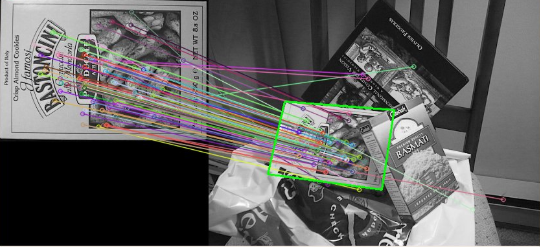
\includegraphics[width=1\textwidth]{section04/assets/RegionRecognition.png}
\caption[Region Recognition Example]{\label{RegionRecognitionExample}Region Recognition Example}
\end{figure}
\par Figure \ref{RegionRecognitionExample} Region Recognition Example shows an example for finding a known object. The book on the left hand side is the object we want to find in the right hand side image. The circles are the keypoints found in both pictures, the lines connect matches found between both images based on the detected keypoints. The green rectangle shows the detected object.
\par Before we begin to detect image features, we need to have a pre-process to call the camera so that we can get each frame to be compared. This will be introduced in Section \ref{CallCamera} Call Camera. The steps and corresponding code to recognize region are listed below:
\begin{enumerate}
\item[1)] Detect the keypoints using {\ttfamily AKAZE} Detector. {\ttfamily AKAZE} is a novel and fast multiscale feature detection and description approach that exploits the benefits of nonlinear scale spaces.\cite{alcantarilla2011fast} This piece of code put the \bsq{\ttfamily ProcessedCamera} image keypoints into \bsq{\ttfamily cameraKeypoints}. \bsq{\ttfamily FeatureDetector} is an OpenCv class used to generate different feature detectors. \bsq{\ttfamily MatOfKeyPoint} is a matrix used to save keypoints.

\begin{lstlisting}[caption={Detect the Keypoints},language={java},
        numbers=left,basicstyle=\footnotesize\ttfamily,breaklines=true,xleftmargin=.05\textwidth, xrightmargin=.05\textwidth]
FeatureDetector featureDetector =
    FeatureDetector.create(FeatureDetector.AKAZE);
MatOfKeyPoint cameraKeypoints = new MatOfKeyPoint();
Imgproc.cvtColor(processedCamera, 
    processedCamera,
    Imgproc.COLOR_RGBA2RGB);
featureDetector.detect(processedCamera, cameraKeypoints);
\end{lstlisting} 

\item[2)] Calculate descriptors (feature vectors). We get \bsq{\ttfamily cameraDescriptor} for \bsq{\ttfamily processedCamera} here. According to an extensive evaluation based on the standard Oxford benchmark \cite{mikolajczyk2005} that shows the excellent compromise between speed and performance of our approach compared to state-of-the-art methods such as BRISK, ORB, SURF, SIFT and KAZE. While A-KAZE is more expensive to compute than BRISK and ORB, it is faster than SURF, SIFT and KAZE.\cite{alcantarilla2011fast}
\begin{lstlisting}[caption={Calculate Descriptors},language={java},
        numbers=left,basicstyle=\footnotesize\ttfamily,breaklines=true,xleftmargin=.05\textwidth, xrightmargin=.05\textwidth]
DescriptorExtractor extractor =
    DescriptorExtractor.create(DescriptorExtractor.AKAZE);
Mat cameraDescriptor = new Mat();
extractor.compute(processedCamera, 
    cameraKeypoints, 
    cameraDescriptor);
\end{lstlisting} 
\item[3)] Matching descriptor vectors using \bsq{\ttfamily BRUTEFORCE\_HAMMING} matcher and only save \bsq{good} matches, the smaller the distance the better the match and here we only use the first half of the matches. 
\begin{lstlisting}[caption={Matching Descriptor Vectors},language={java},
        numbers=left,basicstyle=\footnotesize\ttfamily,breaklines=true,xleftmargin=.05\textwidth, xrightmargin=.05\textwidth]
MatOfDMatch matches = new MatOfDMatch();
DescriptorMatcher matcher =
    DescriptorMatcher.create(DescriptorMatcher.BRUTEFORCE_HAMMING);
matcher.match(cameraDescriptor, 
    giftDescriptor, 
    matches);
            
List<DMatch> bestMatchesList = 
    mats.stream().
    filter( m -> (m.distance - MIN_DIST) < .5 * range)
    .collect(Collectors.toList());
\end{lstlisting} 
\item[4)] Get the keypoints from the \bsq{good} matches. The \bsq{\ttfamily bestMatchesList} is a List of \bsq{\ttfamily DMatch}. \bsq{\ttfamily DMatch} is a data type used to save a match in OpenCv and each \bsq{\ttfamily DMatch} will have the following attributes:
\begin{itemize}
\item distance: This attribute gives us the distance between the descriptors. A lower distance indicates a better match.
\item trainIdx: This attribute gives us the index of the descriptor in the list of train descriptors (in our case, it’s the list of descriptors in the gift images).
\item queryIdx: This attribute gives us the index of the descriptor in the list of query descriptors (in our case, it’s the list of descriptors in the camera capture images).
\item imgIdx: This attribute gives us the index of the train image. 
\end{itemize}
\paragraph{} In our case, we just need first three attributes. The following code shows how we save keypoints into a {\ttfamily LinkedList}, \bsq{\ttfamily objectPoints} will save the gift image keypoints and \bsq{\ttfamily scenePoints} will save the camera capture images keypoints. After we get the keypoints, we will use them to generate the \bsq{\ttfamily homography}. The \bsq{\ttfamily findHomography} method will find a perspective transformation between two planes. The four parameters used in this method are:
\begin{itemize}
\item srcPoints: Coordinates of the points in the original plane, a matrix of the type CV\_32FC2 or vector\textless Point2f\textgreater.(in our case,it's objMatOfPoint2f which comes from gift images)
\item dstPoints: Coordinates of the points in the target plane, a matrix of the type CV\_32FC2 or a vector\textless Point2f\textgreater .(in our case,it's scnMatOfPoint2f which comes from camera capture images)
\item method: Method used to compute a homography matrix.(There are three supported methods, we used RANSAC-based robust method here)
\item ransacReprojThreshold: Maximum allowed reprojection error to treat a point pair as an inlier (used in the RANSAC method only). If srcPoints and dstPoints are measured in pixels, it usually makes sense to set this parameter somewhere in the range of 1 to 10.(in our case, it's three)
\end{itemize}

\begin{lstlisting}[caption={Get Keypoints From \bsq{Good} Matches},language={java},
        numbers=left,basicstyle=\footnotesize\ttfamily,breaklines=true,xleftmargin=.05\textwidth, xrightmargin=.05\textwidth] 
List<KeyPoint> templateKeyPointList = giftKeypoints.toList();
List<KeyPoint> originalKeyPointList = cameraKeypoints.toList();
LinkedList<Point> objectPoints = new LinkedList();
LinkedList<Point> scenePoints = new LinkedList();
    for(int i=0; i<bestMatchesList.size(); i++){
        objectPoints.addLast(templateKeyPointList.get(bestMatchesList.get(i).trainIdx).pt);
        scenePoints.addLast(originalKeyPointList.get(bestMatchesList.get(i).queryIdx).pt);
    }
MatOfPoint2f objMatOfPoint2f = new MatOfPoint2f();
objMatOfPoint2f.fromList(objectPoints);
MatOfPoint2f scnMatOfPoint2f = new MatOfPoint2f();
scnMatOfPoint2f.fromList(scenePoints);
Mat homography = Calib3d.findHomography(objMatOfPoint2f, scnMatOfPoint2f, Calib3d.RANSAC, 3);
\end{lstlisting} 
\item[5)] Put the four corners from the selected region into the template image, in our case, the gift image. Here we use a {\ttfamily Mat} with one column and four rows to record the points. The \bsq{\ttfamily points} is an array of String with user selected region information retrieved from the database, and then, use perspectiveTransform method which performs the perspective matrix transformation of vectors. There are three attributes for this method: 
\begin{itemize}
\item src: Input two-channel or three-channel floating-point array; each element is a 2D/3D vector to be transformed. (in our case, it's templateCorners which comes from gift image.)
\item dst: Output array of the same size and type as src.(in our case, it's templateTransformResult which will save detected corners)
\item m – 3x3 or 4x4 floating-point transformation matrix.(in our case, it's the homography we generated in last step)
\end{itemize}
\paragraph{} After these operations, four corners will be detected to localize the object. The four detected corners of the region is now saved in templateTransformResult.
\begin{lstlisting}[caption={Localize the Object},language={java},
        numbers=left,basicstyle=\footnotesize\ttfamily,breaklines=true,xleftmargin=.05\textwidth, xrightmargin=.05\textwidth]
Mat templateCorners = new Mat(4, 1, CvType.CV_32FC2);
Mat templateTransformResult = new Mat(4, 1, CvType.CV_32FC2);
for(int i=0; i<4; i++){
    templateCorners.put(i, 0, new double[]{points[i*2], points[i*2+1]});
}
Core.perspectiveTransform(templateCorners, templateTransformResult, homography);
\end{lstlisting} 
\end{enumerate}
\par When we first finished the code above, we found out several conditions that could be optimized and we tried to add some factors to constrain the object detected. We put two images in a line and use four-sided shapes to draw both the region selected by user and region detected by the algorithm, after testing thousands of different scenes and manual observation, the factors used to optimize the region are listed below:
\begin{enumerate}
\item[1)] If one of the four corners detected is out of the image bound, that result will be abandoned. 
\item[2)] In case an object matches a very small picture which is not the same, for example, a white board with some lines on it matches a tiny white dot, we add a radio to control the detected object's size. The aspect ratio of the detected region must be greater than or equal to point five times the aspect ratio of  the selected region and the aspect ratio of the detected region must be less than or equal to two times the aspect ratio of the selected region.
\item[3)] The third factor we used is the value of the number of keypoints not in the selected region divided by the number of keypoints in the detected region and both keypoints get from the matches. The smaller factor means a better result. After testing, we decided we only want the result when the factor is less than point three. This factor helps to localize the object.
\end{enumerate}

\subsection{Android Application}
\subsubsection{Usage of Adapter and View}
\paragraph{}
In this project, we used different adapter views in Android to organize different kinds of user interface. An AdapterView is a view whose children are determined by an Adapter. We used \bsq{\ttfamily ListView} to displays a vertically-scrollable collection of views such as gifts list and friends list, where each view is positioned immediatelybelow the previous view in the list. We also used \bsq{\ttfamily GridView} to display the virtual gifts. \bsq{\ttfamily GridView} is a view that shows items in two-dimensional scrolling grid. The items in the grid come from the ListAdapter associated with this view. 
\par As an AdapterView does not know the details, such as type and contents, of the views it contains, AdapterView requests views on demand from a ListAdapter as needed, such as to display new views as the user scrolls up or down.
\par In order to display items in the list, call setAdapter(ListAdapter) to associate an adapter with the list. 
An Adapter object acts as a bridge between an AdapterView (e.g. ListView, Spinner, and GridView) and the underlying data for that view. The Adapter provides access to the data items. The Adapter is also responsible for making a View for each item in the data set. For this project, ListView is used to show friends list and gifts list shown in Figure \ref{FriendsListUI} Friends List page and Figure \ref{GiftsListUI} Gifts List page. GridView is used to show the gifts selection after users choose a region. 

\subsubsection{Get system permissions}
\label{subsubsec:GetSystemPermissions}
\paragraph{} As mentioned in Section \ref{subsec:DatabaseOperations} Database Operations, we need to configure AndroidManifest.xml file. This file is used to declare an application component and declare the permissions that the application needs. As shown below, Line 1 is used to get the internet permission, Line 2 is used to get the external storage permission, and Line 3 is needed to create BmobInstallation. Line 4 is to acquire the system camera permission, we will need this when users send a gift and when users find a gift. Line 5 is used to get user locations. Android offers two location permissions: ACCESS\_COARSE\_LOCATION and ACCESS\_FINE\_LOCATION. The permission you choose determines the accuracy of the location returned by the API. If you specify ACCESS\_COARSE\_LOCATION, the API returns a location with an accuracy approximately equivalent to a city block. However, \bsq{ACCESS\_FINE\_LOCATION} allows an app to access precise location.
\begin{lstlisting}[caption={Get System Permissions},language={java},
        numbers=left,basicstyle=\footnotesize\ttfamily,breaklines=true,xleftmargin=.05\textwidth, xrightmargin=.05\textwidth] 
<uses-permission android:name="android.permission.INTERNET" />
<uses-permission android:name="android.permission.WRITE_EXTERNAL_STORAGE" />
<uses-permission android:name="android.permission.READ_PHONE_STATE" />
<uses-permission android:name="android.permission.CAMERA" />
<uses-permission android:name="android.permission.ACCESS_FINE_LOCATION" />
\end{lstlisting} 
\par The other usage of this file is define an Activity, the code below shows an example. In this example, the Acitivity is named \bsq{SignInActivity} and it is a launcher for this application.
\begin{lstlisting}[caption={Define Activities},language={java},
        numbers=left,basicstyle=\footnotesize\ttfamily,breaklines=true,xleftmargin=.05\textwidth, xrightmargin=.05\textwidth] 
<activity
    android:name=".SignInActivity"
    android:label="@string/title_activity_sign_in">
    <intent-filter>
        <action android:name="android.intent.action.MAIN" />
        <category android:name="android.intent.category.LAUNCHER" />
    </intent-filter>
</activity>
\end{lstlisting} 

\subsubsection{Call Camera}
\label{CallCamera}
\paragraph{} The Camera is another important part in this project. There are two functions which use camera: \bsq{Send a gift} and \bsq{Receive a gift}.
For \bsq{Send a gift} we used system camera. Other than get user permissions mentioned in section \ref{subsubsec:GetSystemPermissions} Get System Permissions, this chunk of code shows an example of calling the system camera. Line 2 to Line 8 creates a file in storage. Line 12 called the system camera and Line 20 saved the picture into the system album. In Line 15 we have a check for sdk version, that is because if the targetSdkVersion >= 24, then we have to use FileProvider class to give access to the particular file or folder to make them accessible for other apps. FileProvider is a special subclass of ContentProvider that facilitates secure sharing of files associated with an app by creating a \bsq{content:// Uri} for a file instead of a \bsq{file:/// Uri}. A content URI allows you to grant reading and writing access using temporary access permissions. 
\begin{lstlisting}[caption={Call Camera},language={java},
        numbers=left,basicstyle=\footnotesize\ttfamily,breaklines=true,xleftmargin=.05\textwidth, xrightmargin=.05\textwidth] 
private void sendMessage() {
    File mediaStorageDir = new File(Environment.getExternalStoragePublicDirectory(
            Environment.DIRECTORY_PICTURES), "giftbox");
    if (!mediaStorageDir.exists()) {
        if (!mediaStorageDir.mkdirs()) {
            Log.d("GiftBox", "failed to create directory");
        }
    }
    String timeStamp = new SimpleDateFormat("yyyyMMdd_HHmmss").format(new Date());
    image = new File(mediaStorageDir.getPath() + File.separator +
            "IMG_" + timeStamp + ".jpg");
    Intent intent = new Intent(MediaStore.ACTION_IMAGE_CAPTURE);
    intent.addCategory(Intent.CATEGORY_DEFAULT);
    Uri uri;
    if (Build.VERSION.SDK_INT >= Build.VERSION_CODES.N) {
        uri = FileProvider.getUriForFile(thisContext, BuildConfig.APPLICATION_ID+".fileprovider", image);//BuildConfig.APPLICATION_ID + ".fileProvider"
    } else {
        uri = Uri.fromFile(image);
    }
    intent.putExtra(MediaStore.EXTRA_OUTPUT, uri);
    startActivityForResult(intent, 0);
}
\end{lstlisting} 
\par After this we will be able to get the result in onActivityResult method. For \bsq{Receive a gift} we use OpenCv to manage the real-time image processing. Other than what we did to get system camera, the extra steps are shown below:
\begin{enumerate}
\item[1)] Extends CvCameraViewListener2 interface in order to use Java API in OpenCv to get the camera preview. There are three methods need to be implemented: onCameraViewStarted, onCameraViewStopped and onCameraFrame. All the important image processing process will be done in onCameraFrame. In our case, this is the place we finish the region recognition.
\item[2)] Add components that display camera content to the interface layout file. Here we will need JavaCameraView to get and display the preview. opencv:show\_fps="true" and opencv:camera\_id="any" options enable FPS message and allow to use any camera on device. Application tries to use back camera first.The following code shows how to do it.
\begin{lstlisting}[caption={Usage of OpenCv Camera},language={java},
        numbers=left,basicstyle=\footnotesize\ttfamily,breaklines=true,xleftmargin=.15\textwidth, xrightmargin=.15\textwidth] 
<org.opencv.android.JavaCameraView
    android:id="@+id/camera_view"
    android:layout_width="fill_parent"
    android:layout_height="fill_parent"
    opencv:camera_id="any"
    opencv:show_fps="true" />
\end{lstlisting}
\item[3)] Declare a CameraBridgeViewBase object to hold the JavaCameraView component in layout file and implement binding and add event listener in OnCreate method. OnCreate method is where we used to initialize the activity.
\begin{lstlisting}[caption={Declare a CameraBridgeViewBase Object},language={java},
        numbers=left,basicstyle=\footnotesize\ttfamily,breaklines=true,xleftmargin=.05\textwidth, xrightmargin=.05\textwidth] 
CameraBridgeViewBase mCVCamera;
mCVCamera = (CameraBridgeViewBase) findViewById(R.id.camera_view);
mCVCamera.setCvCameraViewListener(this);
\end{lstlisting}
\item[4)] Implement the functions we mentioned above. The \bsq{onCameraViewStarted} method is used to initialize the preview images. The \bsq{onCameraViewStopped} will release resources so that the application won't crash. The \bsq{onCameraFrame} method will take care of all image processing, this method will be called every time camera frame refreshed. But because of the algorithm execute takes time so the project result won't be able to show every frame in the result. \bsq{Cur\_State} is used to monitor if the image process begins. \bsq{imageReady} is to ensure the target image is downloaded from database. The \bsq{tag} is used to check if the object has been found.
\begin{lstlisting}[caption={Implementation of Camera Interface},language={java},
        numbers=left,basicstyle=\footnotesize\ttfamily,breaklines=true,xleftmargin=.05\textwidth, xrightmargin=.05\textwidth] 
@Override
public void onCameraViewStarted(int width, int height) {
    mRgba = new Mat(height, width, CvType.CV_8UC4);
}

@Override
public void onCameraViewStopped() {
    mRgba.release();
}

@Override
public Mat onCameraFrame(CameraBridgeViewBase.CvCameraViewFrame inputFrame) {
    if( Cur_State  == 1 && imageReady ) {
        if (tag){
            this.runOnUiThread(new Runnable() {
                public void run() {
                    final Toast toast = Toast.makeText(thisContext, "find it!!!" , Toast.LENGTH_SHORT);
                    toast.show();
                }
            });
        }
        return  compareKeypoints(inputFrame);
    } else {
        return inputFrame.rgba();
    }
  }
\end{lstlisting}
\item[5)]In the above operation, we have already obtained the mCVCamera object in the OnCreate function. After calling mCVCamera.enableView(), the preview component will display the Mat image of each frame, but before displaying it, we must first ensure that the OpenCV library file is loaded. Completed, so calling this method requires asynchronous processing:
\begin{lstlisting}[caption={Load the OpenCv Library},language={java},
        numbers=left,basicstyle=\footnotesize\ttfamily,breaklines=true,xleftmargin=.05\textwidth, xrightmargin=.05\textwidth] 
BaseLoaderCallback mLoaderCallback = new BaseLoaderCallback(this) {
        @Override
        public void onManagerConnected(int status) {
            switch (status) {
                case LoaderCallbackInterface.SUCCESS:
                    Log.i(TAG, "OpenCV loaded successfully");
                    mCVCamera.enableView();
                    break;
                default:
                    break;
            }
        }
    };
\end{lstlisting}
\item[6)] Because only when mLoaderCallback receives the LoaderCallbackInterface.SUCCESS message, it will open the preview display, so we need to override the Activity's onRusume method. Every time the current Activity is activated, this method will be called. so that we can check if the OpenCV library file is loaded:
\begin{lstlisting}[caption={Ensure that OpenCv is Loaded},language={java},
        numbers=left,basicstyle=\footnotesize\ttfamily,breaklines=true,xleftmargin=.05\textwidth, xrightmargin=.05\textwidth] 
@Override
public void onResume() {
    super.onResume();
    if (!OpenCVLoader.initDebug()) {
        Log.d(TAG, "OpenCV library not found!");
        }else{
        Log.d(TAG, "OpenCV library found inside package. Using it!");
        mLoaderCallback.onManagerConnected(LoaderCallbackInterface.SUCCESS);
        }
}
\end{lstlisting}
\end{enumerate}
\subsection{Web Interface}
\paragraph{} The Bmob online database manages user authentication.  Web APIs typically use cookies to store session tokens, but Bmob delivers sesstion tokens to clients via JSON as part of the authentication process.  Our application caches this session token for use throughout the application and delivers the token to Bmob with every subsequent API call after authentication.  
\par Since the session token is not stored as a cookie, there is no need to use CSRF tokens to prevent cross-site scripting attacks. The application is currently insecure as we use HTTP requests to transfer credentials and session tokens to Bmob.  This vulnerability can be fixed by using HTTPS so that all communication with Bmob and with our own Tomcat server will be encrypted. 
\subsection{Conclusion}
\paragraph{} 
In this whole project, more than three thousand lines of code which includes more than twenty classes has been generated for the Android application and eight pages has been generated for the web interface. We also solved some problems like check the sdk version and use \bsq{fileprovider} at proper time to avoid uri exposed exception, add different constrains to get a better detected result and when retrieve data from database, execute the code in main thread and check if data retrieve is finish to avoid asynchronous brings null pointer exceptions.   